\chapter{Resultados entre ligas y en las copas}
\label{cap:rescopas}

\section{La red de ligas (R6)}

\begin{figure}[h]
\centering
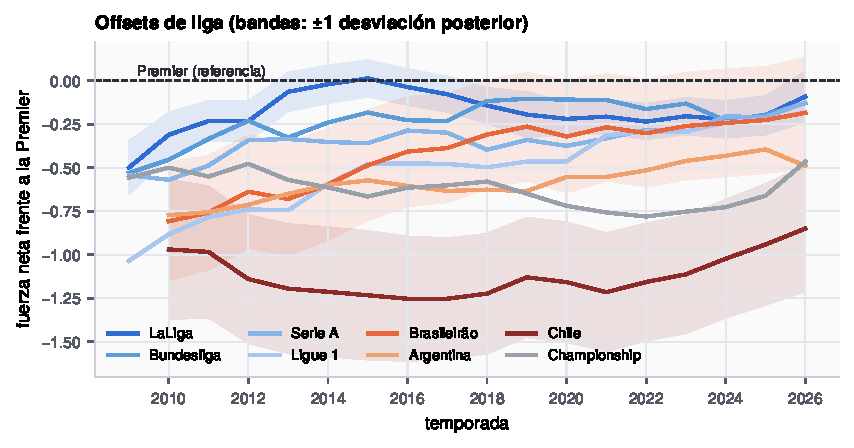
\includegraphics[width=\textwidth]{offsets_ligas}
\caption{Fuerza neta de cada liga frente a la Premier por temporada, estimada con la red de partidos de copa y cambios de división (capítulo~\ref{cap:red}). Bandas de una desviación posterior para LaLiga, el Brasileirão y Chile.}
\label{fig:offsets_ligas}
\end{figure}

Con 2.208 partidos de copa y 611 cambios de división, los offsets netos más recientes frente a la Premier son: LaLiga $-0{,}09$, Serie A $-0{,}13$, Bundesliga $-0{,}13$, Ligue 1 $-0{,}18$, Brasileirão $-0{,}18\pm0{,}32$, Argentina $-0{,}49\pm0{,}35$ y Chile $-0{,}85\pm0{,}37$ (figura~\ref{fig:offsets_ligas}). Las bandas cuentan lo mismo que las resistencias de la sección anterior: las ligas europeas están determinadas con precisión de unas centésimas, y cualquier comparación con Sudamérica tiene una incertidumbre diez veces mayor, porque pasa por el puente del Mundial de Clubes. El ranking global de clubes de la pestaña ``Mundo'' se construye con estos offsets, y por eso cada equipo sudamericano aparece con una incertidumbre mucho mayor que su posición.

\section{Champions League (R20)}

\parrafo{Partidos.} En los 4.100 partidos UEFA de 2018-19 a 2026-27, con hiperparámetros ajustados con 2011-2017, la capa anclada a las 16 ligas con modelo doméstico gana $+0{,}030\pm0{,}004$ nats por partido ($z=7{,}2$) frente a la misma capa solo con partidos de copa, y $+0{,}013\pm0{,}003$ ($z=4{,}4$) frente a la anclada solo a las cinco grandes. La ganancia de las once ligas nuevas está, como debe, en los partidos de sus equipos ($+0{,}024\pm0{,}005$ en 2.093 partidos; en el resto, $+0{,}002\pm0{,}002$). Frente a solo copas, anclar a las cinco grandes ya ganaba $+0{,}018\pm0{,}003$, sobre todo en los cruces entre un equipo de esas ligas y uno de otra (en la Europa League, $+0{,}061\pm0{,}012$).

\parrafo{Torneos.} En ocho ediciones (2018-19 a 2025-26), pronosticadas en ocho o nueve momentos cada una, anclar a las cinco grandes mejora el log score de la etapa alcanzada por cada equipo en $0{,}020\pm0{,}008$ frente a solo copas (siete de ocho ediciones). El del campeón mejora $0{,}11\pm0{,}18$, que es ruido: dos de las ocho las ganó el PSG, con 1,9 y 5,6\,\% al empezar (4,7 y 10,7\,\% solo con copas). Pasar de 5 a 16 ligas es neutro a nivel de torneo ($+0{,}003\pm0{,}005$): el campeón y las rondas finales los deciden equipos de las cinco grandes, que no cambian.

\parrafo{Probado y descartado.} Una media propia para los equipos presentes al empezar los datos y una media común de reversión para los equipos sin liga mejoraban dentro de muestra y empeoraban fuera (log score por partido 2,989 frente a 2,974). Se quedó el modelo más simple.

\section{Libertadores y Sudamericana (R21)}

\parrafo{Partidos.} En los 1.790 partidos de 2021 a 2026, con hiperparámetros ajustados con 2011-2020, la capa anclada a las diez ligas sudamericanas con modelo doméstico gana $+0{,}029\pm0{,}007$ nats por partido ($z=4{,}1$) frente a solo copas y $+0{,}013\pm0{,}005$ frente a la anclada solo a Brasil y Argentina. Con Brasil, Argentina y Chile la ganancia frente a solo copas era $+0{,}018\pm0{,}005$: las siete ligas que se agregaron después para alimentar la capa aportan casi la mitad.

\parrafo{Torneos.} Libertadores 2017-2025 y Sudamericana 2023-2025, pronosticadas al empezar los grupos, tras las fechas 2 y 4, al terminar los grupos y antes de cada ronda: el log score de la etapa alcanzada mejora $0{,}018\pm0{,}008$ por equipo con la capa anclada (ocho de doce ediciones; $0{,}015\pm0{,}010$ en las ocho de 2021 en adelante, las únicas fuera de muestra para los hiperparámetros de la capa). El del campeón, $0{,}03\pm0{,}13$, es ruido.

\section{El nivel de cada liga}

\begin{figure}[h]
\centering
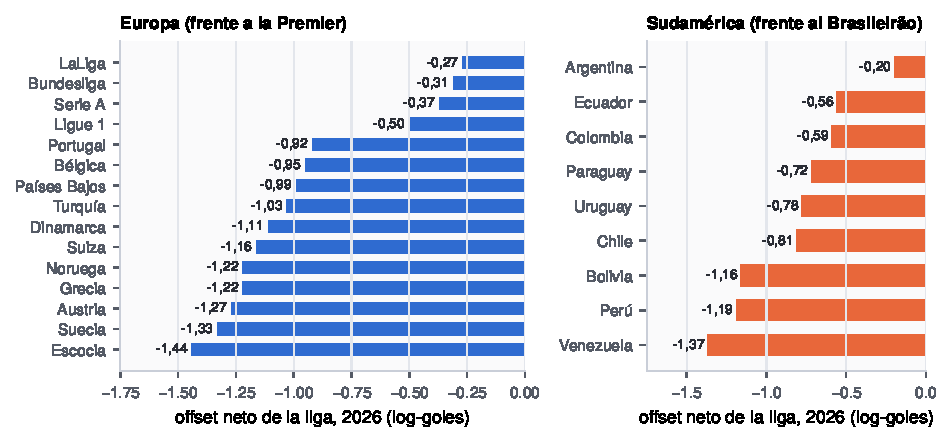
\includegraphics[width=\textwidth]{offsets_copas}
\caption{Offsets netos de cada liga en la capa continental, 2026, frente a la liga de referencia de cada continente. En log-goles: $-0{,}5$ significa que, a igual fuerza doméstica, el equipo genera y recibe goles como si fuera $0{,}5$ log-goles peor que uno de la referencia.}
\label{fig:offsets_copas}
\end{figure}

La figura~\ref{fig:offsets_copas} muestra el nivel de cada liga según la capa. En Europa, las cuatro grandes detrás de la Premier quedan entre $-0{,}27$ (LaLiga) y $-0{,}50$ (Ligue 1), y las once ligas que solo alimentan la capa forman un segundo bloque bastante compacto, de Portugal ($-0{,}92$) a Escocia ($-1{,}44$). En Sudamérica Argentina queda cerca de Brasil ($-0{,}20$) y Chile en el grupo medio ($-0{,}81$), junto a Uruguay y Paraguay. Estos offsets no se comparan directamente con los de la red de la figura~\ref{fig:offsets_ligas}: están en otra escala, porque se suman a una fuerza doméstica trasladada con $\gamma<1$ y conviven con un residuo por equipo y con un nivel de goles propio de cada continente.
